\documentclass[12pt]{article}
\usepackage{wrapfig}
\usepackage{tcolorbox}
\usepackage{hyperref}
\usepackage{titletoc,tocloft}
\usepackage{indentfirst}
\usepackage{setspace,lipsum}
\usepackage{graphicx}
\usepackage{blindtext}
\usepackage[a4paper, total={6in, 8in}]{geometry}
\usepackage[]{sectsty}
\usepackage[T1]{fontenc}
\usepackage[font=small,labelfont=bf]{caption}

\graphicspath{ {./images/} }

\definecolor{lightblue}{rgb}{.68,.85,.90}

\newenvironment{simplechar}{%
	\catcode`\$=12
	\catcode`\&=12
	\catcode`\#=12
	\catcode`\^=12
	\catcode`\_=12
	\catcode`\~=12
	\catcode`\%=12
}{}


%opening
\title{Online Advising Tool}
\author{Jacob Adamsky}


\begin{document}
	\raggedright
	\setlength\parindent{24pt}
	\vspace*{2cm}\setstretch{1}\begin{tcolorbox}[colback=lightblue, colframe=white, width=250pt, height=150pt, center]
		\maketitle
	\end{tcolorbox}
	\setstretch{1.5}
	\begin{abstract}
		\setlength{\cftsubsubsecindent}{12cm} This report represents the work of one or more WPI undergraduate students submitted to the faculty as evidence of completion of a degree requirement. WPI routinely publishes these reports on the web without editorial or peer review. In an effort to improve the digestibility of both the graduate and undergraduate catalogs, this project aimed to re-imagine how students are able to access the course requirements for their degrees. Unlike the current system for seeing the course requirements for your degree, the new system allows students to create a mock schedule, giving them a general idea of when they will be taking courses in the future.
	\end{abstract}
	
	\pagebreak
	\tableofcontents
	\pagebreak
	
	\section{Setting Things Up}
		\subsection{Downloading the Application}
			The first piece of software to install is Visual Studio (not VS Code). You can find the download for it \href{https://visualstudio.microsoft.com/downloads/}{here}. If you have access to a Professional or Enterprise license, you can go ahead and install that. Otherwise, stick to Community because it's free with your WPI email, while the other two will expire in 30 days. The second piece of software you'll want to install is MySQL Workbench (if you have your own preference for managing the MySQL database, use that instead). This isn't entirely necessary, but can be very helpful if you're adding data to the database and make an error as it allows you to quickly fix it without re-entering everything. The download for that can be found \href{https://www.mysql.com/products/workbench/}{here}.
			Lastly, you'll want to download the actual web application. All relevant files for the project can be found 
			\href{https://github.com/adamskyjacob/Advising-Tool}{here}. The connection string in Utils.cs is missing the server and password, so all you have to do is follow the instructions in the Account and Database section.
			
		\subsection{Setting Up Microsoft Azure}
			The first step to begin setting up the application is to create a free Microsoft Azure account and log in \href{https://azure.microsoft.com/en-us/}{here}. Next, click on the "App Services" button towards the top-left of your screen and create a new app service. Once you've been redirected, create a resource group, pick a name for your instance, select .NET 6 (LTS) for the Runtime Stack, and then click Create at the bottom left of your screen. This part may take a few minutes, so it would be best to move onto setting up things in AWS.
			
		\subsection{Setting Up AWS and RDS}
			\subsubsection{Account and Database Setup}
				To start with AWS, head to \href{https://aws.amazon.com}{this} page and create an AWS account, making sure to not choose any options that will cause unwanted billing to your account (it's possible that Amazon would waive the fees if you mentioned you were working on a school project). After logging in as the root user, search for RDS in the and click on the first result labeled "Managed Relational Database Service". Head to the Databases tab which can be found on the left menu and create a database. Select standard create, MySQL for the engine option and the latest engine version, free tier for the template so you don't get billed, and set the DB instance identifier to advising. Choose a new master username and master password (don't use anything private as this will be visible to anyone who works on the project in the future), set the storage type to gp2 and the allocated storage to 20 GiB, allow public access, and create a new VPC security group in any of the three us-east zones. Once the database has finished creating, go back to the main RDS databases page and open your database. Under Connectivity \& security, copy the endpoint which will look something like 'advising.(some random stuff).us-east-2.rds.amazonaws.com, open the Utils.cs file inside of the project downloaded 
				\begin{wrapfigure}{r}{0.3\textwidth}
					\vspace*{-.6cm}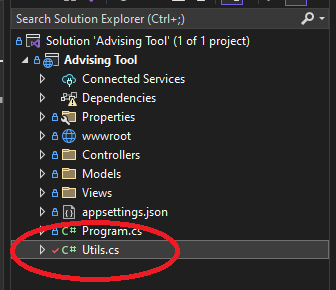
\includegraphics[scale=.45]{utilslocation}
				\end{wrapfigure}earlier (path is /Advising Tool/Advising Tool/Utils.cs), and replace the server with your endpoint (leave the ,3306), the user with your admin username (if you picked a new one), and password with your password. The figure to the right shows where Utils.cs is in Visual Studio. With every folder collapsed, it should be the last file.
				
			\subsubsection{Installing MySQL Workbench}
				Launch MySQL Workbench and click the + button next to "MySQL Connections". Name the connection something along the lines of Advising Tool, set the hostname to the endpoint from your RDS database, the username to your database admin username, and then click OK. After the popup disappears, click on the database instance and enter your password. If you get a connection error, make sure you followed all the previous steps correctly, and that the VPC security group you have linked to your database has both an inbound and outbound rule for MYSQL/Aurora with the TCP protocol and 3306 as the port.
				
			\subsubsection{Setting up the Database}
				To start, right click on the schema called sys and click "Drop Schema". This schema holds no important information, so click OK. Right click on the empty SCHEMAS section and Create Schema with the name advising. For each file in "Database CSV Files", right click on the "Tables" section, click "Table Data Import Wizard", browse to the CSV file, select it and click next, create a new table with the same name as the file you are currently importing (excluding file extensions). Once all of the tables have been imported, you're ready to hook everything up to Microsoft Azure.					
				Note: AWS RDS can and will be very slow. It can take anywhere between 5-15 seconds to load a page, so try not to close out of tabs before they load or swap tabs too frequently while others are loading.
				
			\subsection{Visual Studio and Microsoft Azure}
				For this part, you'll need to log into Visual Studio with the same email you used for Microsoft Azure. Once you've done that, open up "Advising Tool.sln" and open the "Build" menu on the top bar. Select "Publish Advising Tool" and create a new target at Azure. Click next, select Azure App Service (Windows), select Azure instance you created in the first part, and select the "Publish (generates pubxml files)" option. Once that is finished, click on the Publish button at the top of your current screen. Visual Studio will automatically open a browser window with the application's website, but you'll need to add "/Home" to the end of the link to access the website. With that, you should be good to look around the website and start modifying it as you see fit. To update the website, simply click the "Publish" button again. 
				
	\pagebreak
	\section{Using the System as an Administrator}
		\subsection{Administration Access}
			Currently, no there are no login credentials to determine who has access to the Administration page, which can be accessed from the top-left hamburger menu. Once you enter the Administration page, there are four different options you can choose from: Add Undergraduate Course, Add Undergraduate Sheet, Add Graduate Course, and Add Graduate Sheet. Both the course and sheet pages work identically to each other, so I'll explain from the perspective of someone adding to graduate side of things.
		
		\subsection{Adding a Course} 
			\begin{wrapfigure}{r}{0.3\textwidth}
				\vspace*{-1.3cm}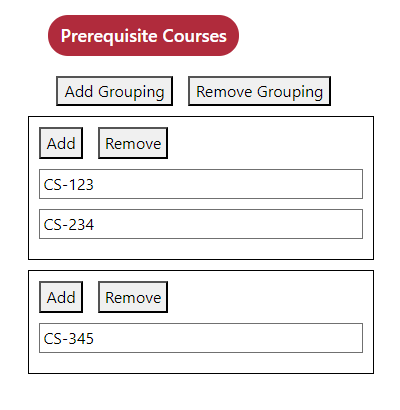
\includegraphics[scale=.6]{prereqexample}
			\end{wrapfigure}
			At the moment, course area is a text entry, but should be updated to be an HTML select instead. First, you pick the course area, enter the course ID (1001, 1002, etc.) and course name,the description, and how many credits its worth. For undergraduate courses, enter the credit value as a fraction e.g 1/3, 1/6, while for graduate courses, enter a whole number depending on what the catalog lists the course credits as. For prerequisite and recommended courses, you'll want to add a new grouping for each prerequisite course. For  example, in the image to the right, courses CS-123 and CS-234 are in a group together, meaning someone who is selecting courses can pick CS-123 OR CS-234, not both. Each course group must have a course selected from it, otherwise the student will get a warning about missing a prerequisite (prevents them from adding the course to a schedule) or a recommended background warning (just an alert popup, still allows course to be added to schedule). Next, there is an option "Credit Range" input for the course. This is used in the case that a course has a variable number of credits, e.g. RBE 598 Directed Research can have up to 9 credits as an elective course. Lastly, tehre is the "Waive Options" section which is use in conjunction with "Waive Course Form URL". Here, you can add an option to take the course at the same time as another (in the case that this isn't normally allowed), or you can choose to waive the course requirement entirely, replacing the course instead with degree-related electives. You also should include a link that directs students to a waiver form for all options you've added here.
			
		\subsection{Adding a Tracking Sheet}
			Adding a tracking sheet is a more complex task. Depending on what the course requirements are, you'll have to use each section to the best of it's abilities. First, enter the degree area (which, like in adding a course, should be an HTML select), the full name of the degree, and the degree ID (e.g MS for Master of Science). Do note that some degrees have widely different course requirements depending on the final option you select, so it may be best to make a whole other tracking sheet instead of adding multiple options to the "Final" section. Free electives represents the number of credit hours (graduate) or units (undergraduate) a student can take in whatever area of study they please, while degree-related electives must be in the student's area of study and committee-approved electives must be approved by the graduate committee (only for graduate sheets). For "Course Sections", treat the course groups similarly to those in adding a course prerequisite -- you can only select one course from each group. Focused electives are electives from a specific list of areas (this should also be modified to be an HTML select instead text inputs). Specialty areas allow a student to select up to n number of course sections for their degree specialty (only been used in Business degrees). As for a Depth area, they are very similar to Specialty areas and Course Sections, except for the fact that a student can only pick one of the Depth sections for their degree. Lastly, there is the Final entry. How you enter the data for this is entirely dependent on the course requirements for each final type. Some study areas have the same course requirements for thesis vs. non-thesis degrees, while others vary to the point that multiple tracking sheets are necessary. Each final option can have multiple groups of course sections depending on what is necessary to complete the degree, and each course section can either have a credit range or a number of times the course must be taken. Do note that students cannot add courses in a final section to anywhere in their schedule -- it is only visible on the final selection page or once you download the schedule as a PDF.
			\par
			Note: For all undergraduate credit inputs, only enter fractional values unless the course units are a whole number. For all graduate credit inputs, only enter whole numbers. Doing otherwise will lead to a non-functional tracking sheet.
			
	\pagebreak
	\section{Working with the Catalogs}
		\subsection{Regular Expressions and Data Validation}
			This part of the process only took a couple of days to get done. From each catalog, I copied every course entry and pasted them into Notepad++ (also used Visual Studio for JSON formatting). From there, I used "Find", set to regular expression with ". matches newline" off, to search with three different regular expressions. 
			\begin{simplechar}
				Firstly, I used '([A-Za-z]+) ([0-9]+): ([A-Za-z\-\/. ]+)' as the find query to locate the area, ID, and name of the courses and set the replace expression as '\{"AREA" : "\$1", "ID" : "\$2", "NAME" : "\$3", "DESC" : "'. Each \$# in the replace expression corresponds to a parenthesis-contained regular expression (\$1 => ([A-Za-z]+)). After separating all of this data, the next regular expression Find query was 'Credits: ([0-9]+)' and the replace statement was '", "CREDITS" : "\$1" \},'.
			\end{simplechar} 
			For courses without credits listed, I manually added a CREDITS property in the JSON for the course and set it to "0". Alternatively, the MySQL Workbench JSON import could have manually entered NULL values, but I avoided this so I didn't have to worry about handling them. The last regular expression I used was to remove the catalog page numbers. The find query was 
			\begin{simplechar}
				'[0-9]+ .* Catalog' and the replace statement was '' (empty string). After all that, I saved the file as a .json and opened it in Visual Studio where I used two quick regular expressions of '\textbackslash n' and '\textbackslash r'
			\end{simplechar}to find and remove all newlines in the document. Splitting the regular expressions apart instead of doing something like '[\textbackslash n\textbackslash r]*' was necessary as doing it like this caused Visual Studio to crash. Once all newlines have been removed, I used CTRL + K, CTRL + D to auto-format the document, and then I scrolled through the file to make sure all courses had an AREA, ID, DESC, and CREDITS property. Whenever necessary, I made corrections to the course information due to the regular expressions being an imperfect solution. Unfortunately, there was no effective way for either undergraduate or graduate courses to enter prerequisite and recommended background courses, so I had to manually enter the data for all course that had this attribute.
			
		\subsection{Entering Tracking Sheets}
			I started with entering the graduate degrees as I knew this process was going to be a bit more difficult than the undergraduate side. Not all graduate degrees had a clear-cut course track, so for those without a clear plan, I didn't enter them into the database. As for undergraduate tracking sheets, most, if not all degrees have a well-organized tracking sheet, so this process went a lot quicker.
			
	\pagebreak
	\section{Development and Testing}
		\subsection{Pre-Development}
			Before I had started development of the course and tracking sheet entry pages, I knew I needed to come up with a plan on how I was going to store the data. After selecting a database hosting service (I explained how to set up AWS RDS above, but personally used Azure MySQL hosting in the hopes of faster speeds, which I was unfortunately not graced with), I opened up a blank JSON file and started coming up with a general structure for how I was going to enter the data. Once I had come up with a basic format, I created the Add Tracking Sheet page for graduate sheets (did this first because I knew it would be more difficult to do data entry) and entered the majority of the degrees I could. The next step was to process the data, and ASP.NET worked wonders. As the .cshtml pages supported both HTML and a slightly modified version of C\#, I was able process the data entirely server-side. All of this, and the fact that I am fairly familiar with C\#, were the main reasons why I chose to use ASP.NET over React and JavaScript (on top of the fact that I got an error trying to use MySQL with React with no solutions online).
		
		\subsection{Development}
			Originally, I was planning on using JavaScript and React as my framework, but as I previously mentioned, I couldn't get React to work on my system.. Initially, I set up all of the containers and navigation bars that would be needed, and then I started parsing all of the information with C\#. What I should have considered first while doing this was how I was going to keep track of the required credits for each section of the degree, but I dealt with that later. Once all the raw HTML elements were on the pages for courses, sections, etc., I set up CSS style sheets for each view and tinkered with them until I got a relatively decent-looking page. The next step was writing all the JavaScript functions to do credit calculation, section hiding, navigation, and prerequisite / recommended background / section credit checks. Because of how some of the divs were organized in the raw HTML, I had to do several element class and ID checks to make sure the correct element was being modified. As for the navigation and section hiding, that process was extremely easy and very straight forward. Simply document.querySelector the section you want it visible, set it's hidden attribute to false, document.querySelectorAll all of the sections that should be hidden, and set them to hidden. The same went for minimizing and maximizing course sections (when possible).
			
			\subsubsection{Implementing Schedule Downloading}
				\paragraph{Initial Implementation:}
					Without use of an external package, the only option I had to enable saving the course schedule was to use the print function in JavaScript. This allows you to create a variable that you can write simple HTML to with inline CSS, and then print the element as if you were printing to a printer, but instead of printing to a printer, you would select "Print to PDF" and save the file locally. While it isn't the prettiest solution, I would definitely say it was very effective in getting the job done. One benefit to this solution, though, is that you could querySelector a specific element you wanted to add to the downloaded PDF, .cloneNode(true) on it, remove any unnecessary or undesired child elements, and then add element.toString() to the print string.
				
				\paragraph{Final Implementation:}
					A simple PDF form package called "pdf-lib" was freely accessible online, so I imported the script using a \begin{simplechar}<script src="..."></script>\end{simplechar} element in HTML. This script allows you to import a locally stored PDF as a JavaScript variable, and modify the form values by selecting them based on their hidden input tags. This made it very easy to export the course schedule as a Plan of Study PDF.
					
		\subsection{How it Works}
			Something to note about HTML element dataset attributes is that they are always stored as strings, so you must explicitly convert the dataset value to the desired type. For example, if you are trying to access the prerequisite data array, you must do JSON.parse(value) to convert it to an array as there is no other explicit conversion in JavaScript from a string to an array. The same thing goes for every other datatype you wish to store, no matter how basic (integer math doesn't work consistently if you don't convert).
			\subsubsection{\texorpdfstring{C$\#$ and JavaScript}{}} 
				\paragraph{C$\#$:}
					To get all of the courses visible on the website, C\# was used in conjunction with HTML to dynamically create HTML elements with the data received from the MySQL database. With each function call (e.x. GetCatalog() or GetUGCatalog()), the website's server creates a connection to the database and queries for the desired course entries. The resulting rows are then converted into the Course model (Course.cs in models) and added to a list of courses. In certain sections (e.x. core electives, non-core electives), the courses are filtered which can be done very easily with an (Object).Where(course => course.property == true) call to return an array with matching courses. Once all of the course sections are populated, the rest of the functionality is entirely in JavaScript. 
				 
				\paragraph{JavaScript:}
					The rest of the site functionality will be explained here. The three most important JavaScript functions used when adding and removing courses are modifyCourseScheduling, updateCreditCount (or corresponding function depending on parent section type), and downloadSchedulePoSPDF. 
				\paragraph{modifyCourseScheduling:}
					The modifyCourseScheduling function handles almost all of the logic for adding courses to the Selected Courses page (as well as removing them when a course is deselected), with the exception of the final project selection which is handled by addFinalCourse (this function works very similarly to when you call modifyCourseScheduling on a course with a credit slider). When the courses were initially added to the page, they included their dataset values (recommended background, prerequisites, min-max credits if needed, course area and id, and a copy of the course prerequisites). Both the recommended background and prerequisite data values are used to check whether or not the necessary courses have been added to previous semesters on the schedule. If not, the course has a boolean attribute (for prerequisite) set so that the stylesheet turns it yellow, indicating that you are missing a prerequisite course (you also get an alert with window.alert), or just a window.alert if you are missing recommended background. Additionally, when you select a waive option for RBE500, the course prerequisite data will be modified to remove RBE 500 as a prerequisite, or if you chose to take RBE 501 or 502 with RBE 500, RBE 501 or 502 will be added to the sametime data array which is then used to check whether or not the semester the course is being added to includes the course you elected to take with RBE 500. If not, you get an alert just like with recommended background. A check is also performed on all courses using checkPrerequisite and checkRecommended which will alert the user if a prerequisite or recommended background course has been removed from scheduling. 
				\paragraph{updateCreditCount:}
					Each corresponding updateCreditCount or similar function adds to the courses parent section's credit (or credits) data value the correct amount of credits from the course when you select it. Another function is used for the global credit counter which happens with the updateGlobalCredits function. When a course is selected, if the credit count equals or exceeds the required credits for the given section, all non-selected courses in the section are disabled, preventing the user from selecting more courses. The section credits are used when users attempt to access the Advisor Approval page: if the credit threshold for all sections hasn't been met, you can't access the page.
				\paragraph{downloadSchedulePoSPDF, getScheduleForEmailHTML:}
					I consider downloadSchedulePoSPDF to be one of the most important functions as it allows students to download their plan of study to the official WPI RBE Plan of Study PDF, with the ability to add all of your personal information and automated adding of courses and final selection to the PDF in one place. This might not be a massive time save, but in terms of convenience, I think this is one of the nicest features of the website. Students are still required to manually sign and date the plan of study PDF, but this is a feature that could be added by whoever works on this next. Additionally, there are more detailed text entries for the MS Thesis option, so the data entry popup could be modified to include those as well.
					\par
					getScheduleForEmailHTML and getScheduleForEmail (child function not listed in title) are both used together, allowing the user to click on a button and open up an email window (with the system email application) that already has the currently selected schedule in the body. It also lets you had a custom message, and shows a preview of what the email will look like before it's opened in a new window.
				\paragraph{Remaining Functions:}
					The remaining functions not explicitly listed here likely function very similarly to previously mentioned functions, or serve very basic purposes such as adding or removing values to an elements dataset values.
				
		\subsection{Testing}
			When I started this project, I had the database and the ASP.NET server running locally, so SQL queries were a lot quicker and the website loaded a lot faster. This made testing very easy for me as the process was basically: add a new function to JavaScript, test it's functionality on an actual tracking sheet, and fix any issues that arose. Where testing became a bit of a nightmare was once I linked my Visual Studio project and the database to Microsoft Azure. As I mentioned previously, loading times with the free database and server hosting are not particularly fast. On top of the 5-15 second loading times for the website, I had to wait another 20-30 seconds for the publish to Azure to go through, and it wasn't even guaranteed for the change to fix the issue. I strongly recommend keeping a local database instance (that is kept up-to-date with the RDS database) and figure out a way to select between the local and server SQL connection strings to avoid the slow loading times while testing. A lot of credit for bug/issue testing goes to Professor Agheli, as well as a couple of friends.
	
	\pagebreak
	\section{User Experience}
		\subsection{Undergraduate and Graduate Scheduling}
			Both undergraduate and graduate course scheduling work virtually the same. The main difference between the two is that all undergraduate majors have a "Project-Based Learning" section which contains IQP, MQP, and HUA. Both IQP and MQP contain an empty placeholder course called IQP-1 and MQP-1 respectively just so the students have something to select during scheduling.
			\par
			The scheduling process is pretty straight-forward. After picking the your area of study and the specific degree you want to receive, you are redirected to the course scheduling page. Most, if not all, degrees will start you off on the Course Selection tab with General courses selected. Regardless, the process is the same. Look through the course options for each section and pick whichever ones you find interesting (course information can be seen by clicking on the course label) while still meeting the credit requirement. Some courses have waive options, so select those as desired. It is advised that you select all courses for your general courses before moving on to electives because there is a chance you may select the only available option in a course section while selecting 
			\begin{wrapfigure}{r}{0.35\textwidth}
				\centering
				\vspace*{-1.2cm}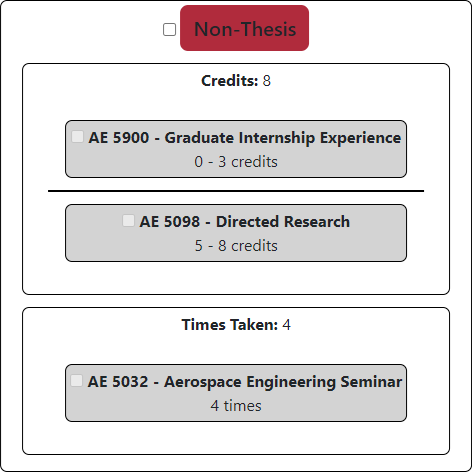
\includegraphics[width=6cm]{creditexample}
			\end{wrapfigure}degree-related electives. Once you've selected enough credits from each section, you can then pick your final option. Some degrees don't have a final requirement (dissertation, capstone), so this isn't always applicable. Each final can have multiple sections of courses to select from, and it's important to note that some course options in the final selection page have a credit range instead of a single number. For example, the picture on the right shows the Aerospace Engineering non-thesis final option. The credit requirement for the first section is only 8 credits, but with the way the system works, the maximum number of credits will be picked from each selected course and added to the course counter. In the future, this could be modified to ensure that the global credit counter does not get updated past the limit of each section, as selecting both options currently adds 11 to the credit counter instead of 8. Lastly, certain courses (e.x. RBE 594, RBE 596, RBE 598, RBE 599) can be split up into multiple sections depending on how many credits you have elected to take for them.
			\par			
			To start organizing your courses into a semester-based (graduate) or term-based (undergraduate) schedule, you can go to the selected courses tab. If you are missing credits from any given section, or forgot to select a final option, you will get a popup listing all of the areas you are missing selections in. Once you get into the scheduling page, you can start selecting courses and adding them to semesters. If you try adding a course to your schedule and you are missing prerequisites for that course, you will get a popup telling you what courses you are missing and you wont be able to add the course to your schedule. The same goes for recommended background courses, but you can still add the course to your schedule. If you have already taken a prerequisite course, for an undergraduate degree for example, you can type the course in the format of MA-1021 (hyphen separating area and course ID). Once you are done with scheduling, you can download the Plan of Study for your degree, which will have your selected final option, as well as your selected courses, already filled out. Additionally, once all course section requirements have been met, you can proceed to Advisor Approval where you can generate a template email for an advisor.
				
		\subsection{General Graduate Scheduling}
			General scheduling is currently only available for graduate courses, but it functions very similarly to how regular course scheduling works. You can search through all courses in the graduate catalog, and pick whichever courses you'd like with no restrictions. They can then be added to the same semester-based calendar that you'll find in the graduate course scheduling. 
		
		\subsection{Course Catalogs}
			Both undergraduate and graduate courses can be accessed through their respective course catalog pages. There, you can click on a course and view it's information including the course description, credits, recommended background, and prerequisite courses. There are also two search options: title search and description search. You can enable both to search course descriptions and titles for content, or you can choose just one. If you have none selected, the search input does nothing. You can also filter courses based on their study area
		
		\subsection{Help Page}
			This section will be intentionally brief. As there are currently no security measures to prevent SQL injection attacks (however unlikely they may be, especially with how the site is being hosted) there is an issue submission form on the help page in the case that students see any content that is unintended or was injected by an external user. Future iterations of the system could have a feature that allows students to make proposed changes to the database (modifying a course description, prereqs, etc. or a tracking sheet course requirements, name, etc.) which could then be accepted or rejected by a system admin.

	\pagebreak
	\section{File System}
		\subsection{Controllers}
			This folder is where you can add/remove more controllers. The controllers for an ASP.NET application (at least how I used them) are primarily for SQL updates and natively used for URL routing. For example, the method
			\begin{wrapfigure}{r}{.45\textwidth}
				\centering
				\vspace*{-.55cm}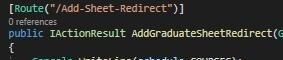
\includegraphics[width=1\linewidth]{images/routeexample}
			\end{wrapfigure} AddGraduateSheetRedirect in the picture to the right would have a default path of "/Home/AddGraduateSheetRedirect", but because of the [Route("/Add-Sheet-Redirect")], this specific view now has the route of just "/Add-Sheet-Redirect". For every .cshtml file you have in the "/Views/Home" folder, you need a corresponding method that returns an IActionResult in the controller. If the name of the .cshtml is different than the method name, the page will fail to load.

		\subsection{Models}
			Models are just normal C\# classes which are used as the model proprety of a .cshtml file. They are necessary, especially when making a SQL insert or update call, as the ASP HTML form used to submit the data to HomeController.cs requires each input to be a property of the Model class. Otherwise, the data submitted by the form won't be sent to the controller and will never be part of a SQL query. Instead of using fields in the class, the model must exclusively use properties (these have getters and setters). ASP.NET requires this for any class which is used as a model.
			
		\pagebreak
		
		\subsection{Views}
			The last aspect of the file structure is Views. This is where the data from the Model is processed and turned into HTML and JavaScript. It's important to note that, while you can pass data from C\# to an HTML attribute (e.g. set dataset-num=@course.CREDITS), you cant do something like
			\begin{wrapfigure}{r}{.32\textwidth}
				\centering
				\vspace*{-.75cm}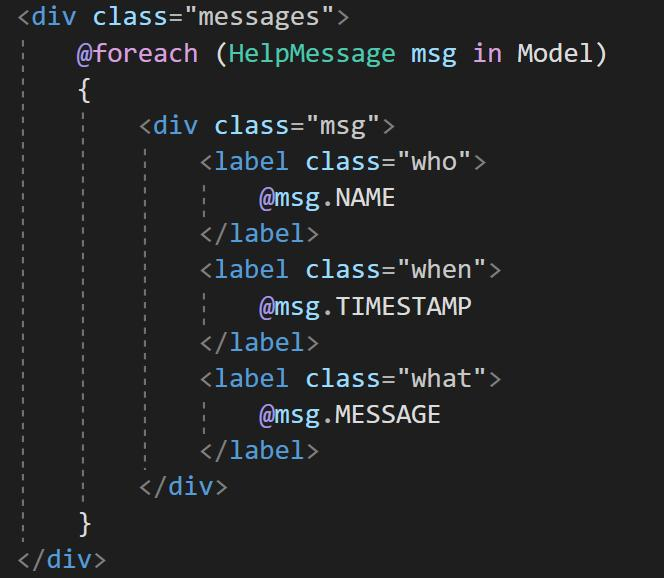
\includegraphics[scale=.3]{cshtmlexample}
			\end{wrapfigure} onclick=@GetCourseInfo(this). As all C\# is run server-side, you can't pass any data from JavaScript or HTML into a C\# function. As you can see in the example .cshtml code on the right, all C\# method calls when processing must be preceded by an \@. This is so you can distinguish between HTML elements and their text, and the C\# method calls. One exception to this is if you are currently inside the scope of a C\# loop, or if you are inside of @\{\}, the latter allowing you to put whatever C\# variables you want inside. All views must have a corresponding IActionResult method in a controller (method name must be identical to file name preceding file extension).
			\subsubsection{Shared Views}
				Shared views are an easy way of having identical HTML be displayed on multiple pages without having to copy over the same code. The \_Layout.cshtml that I wrote up for this project includes the header, the page up button, and the side menu. For the purposes of this project, I didn't look into how to use shared views for different pages, so there may be a way to do a shared view for certain pages here to limit duplicate code.
\end{document}
